

%%% Uncomment for slide version
\documentclass{beamer}
\setbeameroption{hide notes} % Only slides

%%% Uncomment for handout version
%\documentclass[handout]{beamer}
%\setbeameroption{show notes on second screen=right} % Both

\setbeamertemplate{note page}{\pagecolor{white}\insertnote}

\setbeamertemplate{footline}{}

\usetheme[progressbar=frametitle]{moloch}% modern fork of the metropolis theme

\setbeamercolor{background canvas}{bg=white}
\setbeamercolor{progress bar}{use=palette primary,fg=red,bg=red}

\setbeamercolor{note page}{bg=white} 

\setbeamertemplate{date}{}


\defbeamertemplate*{title page}{customized}[1][]
{
	\usebeamerfont{title}\inserttitle\par
	\bigskip
	\bigskip
		\bigskip
			\bigskip

	\usebeamerfont{title}\usebeamercolor[fg]{subtitle}\insertsubtitle\par
	\bigskip
	\usebeamerfont{author}\insertauthor\par
	\usebeamerfont{subtitle}\insertinstitute\par
	\usebeamercolor[fg]{titlegraphic}\inserttitlegraphic
}

\addtobeamertemplate{navigation symbols}{}{%
	\usebeamerfont{footline}%
	\usebeamercolor[fg]{footline}%
	\hspace{1em}%
	\insertframenumber/\inserttotalframenumber
}
\setbeamercolor{itemize item}{fg=black}
\setbeamercolor{itemize subitem}{fg=black}
\setbeamercolor{itemize subsubitem}{fg=black}

%%% Slide 1

\title{\Huge FRST302: Forest Genetics}
\author{\Large Lecture 1.1: Classical Genetics and its Molecular Mechanisms}
\date{\today}

\begin{document}
	\maketitle

\note{\emph{Remember, everything on the lecture slides and the accompanying notes is potentially examinable!}}
% for the beamer version
%\documentclass{beamer}

%%% Slide 2
	
	\begin{frame}

\Huge \centering \emph{What are the major genetic questions in biology?}
\vspace{20pt}
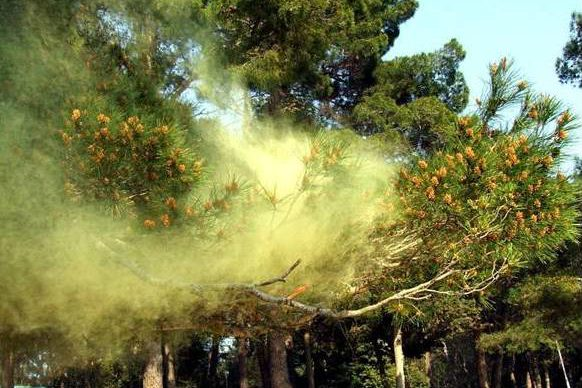
\includegraphics[keepaspectratio, width  =0.9\textwidth]{img/pollenPlume}
   \note{
   	The answer to this question totally depends on your perspective. However, I think that it is more than fair to say that the following questions are at the heart of most biological science:
		\begin{itemize} 
			\item Why is there so much variation among individuals?
			\item How is this variation maintained in populations?
			\item Why do offspring tend to resemble their parents? 
					\par
		\end{itemize}

		\footnote \url{https://www.asthmacenter.com/wp-content/uploads/Pine-Pollen-Plume-e1495119706845.jpg}
	}
	\end{frame}

%%% Slide 3
	
\begin{frame}
		\frametitle{Outline for Today}
\setbeamertemplate{itemize items}[circle]
\Large{
			\begin{itemize} 
			\item Basic definitions in genetics
			\item Principles and terms in classical genetics
			\item Molecular mechanisms of classical genetics
			\item Recombination and its significance
		\end{itemize}
	}

\note{
Learning Outcomes
	\emph{		\begin{itemize} 
				\item Basic definitions in genetics
				\item Principles and terms in classical genetics
				\item Molecular mechanisms of classical genetics
				\item Chromosome crossover and its significance
			\end{itemize}
	}
}
\end{frame}

%%% Slide 4
\begin{frame}
\frametitle{History of Genetics}

\Large \textbf{What is genetics?} \par

\bigskip
\pause
\Large \textbf{Genetics is the study of genes}, of variation and heredity across all branches of the tree of life




\end{frame}


\begin{frame}
	\frametitle{History of Genetics}
	
\begin{columns}[T]
	\begin{column}{.7\textwidth}
			Humans have probably pondered inheritence for all history:
			\vspace{10pt}
			\begin{itemize}
				\item The Ancient Greeks considered Male and Female 
			\end{itemize}
	\end{column}
	\begin{column}{.3\textwidth}
			% Your image included here
% TODO: \usepackage{graphicx} required
\centering
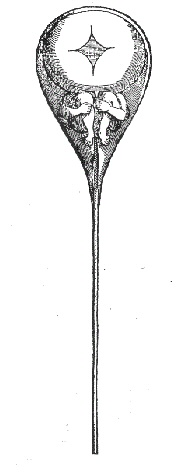
\includegraphics[keepaspectratio, width  = 0.8\textwidth]{img/homunculous}\footnotemark[1]


	\end{column}
\end{columns}

\footnotetext[1]{\url{https://en.wikipedia.org/wiki/History_of_genetics}}

		
\end{frame}




\end{document}